\chapter{Generalized Linear Model (GLM)}
\label{ch-gen-lin-mod}

This chapter is based on
chapter 4 of Ref.\cite{agresti-book}.

\section{Exponential Family of Distributions}
\label{sec-exp-fam}

The {\bf Exponential Family (EF)} of probability distributions is defined by

\beq
P(y|\theta, \phi) =
\exp\left(\frac{\theta y - b(\theta)}{a(\phi)}+c(y,\phi)\right)
\eeq

In this chapter, we will
denote averages over $y|\theta, \phi$ by angular brackets

\beq
E_{\rvy|\theta, \phi}[f(y)] = \sum_y P(y|\theta, \phi) f(y) = \av{f(y)}
\eeq
As usual in this book, let $S_\rvx$ denote the set of
values that the random variable $\rvx$ can take.
We will assume that $S_\rvy$
for EF
can be either a discrete or a continuous
subset of $\RR$,\footnote{By a \enquote{continuous set} we
mean a finite set of intervals
 each of which has non-zero length.}
but $S_{\ul{\theta}}$
must be continuous.
When $S_\rvy$ is a discrete subset of $\RR$, $P(y|\theta, \phi)$
will denote a probability distribution, whereas when
$S_\rvy$ is continuous, it will denote
a probability density.

\begin{claim}
\beq
\mu = \av{\rvy} = b'(\theta)
\eeq

\beq
\s^2= \av{\rvy, \rvy} = a(\phi)b''(\theta)
\eeq
\end{claim}
\proof

\beqa
0&=& \partial_\theta \int_{-\infty}^\infty
dy\; P(y|\theta, \phi)
\\
&=&
\int_{-\infty}^\infty
dy\;\frac{1}{a}
[y-b'(\theta)]P(y|\theta, \phi)
\\
&=&
\frac{1}{a}[\av{\rvy}-b'(\theta)]
\eeqa

\beqa
0&=& \partial^2_\theta \int_{-\infty}^\infty
dy\; P(y|\theta, \phi)
\\
&=&
\int_{-\infty}^\infty
dy\;\left\{\frac{-b''(\theta)}{a} +
\frac{1}{a^2}
[y-b'(\theta)]^2\right\}
P(y|\theta, \phi)
\eeqa
Hence,

\beq
\av{[y-b'(\theta)]^2}= a b''(\theta)
\eeq

\qed

Note that the Normal Distribution
belongs to the EF. Indeed,

\beqa
\caln(y; \mu, \s^2)
&=&
\frac{1}{\sqrt{2\pi \s^2}}
\exp\left(
-\;\frac{(y-\mu)^2}{2\s^2}
\right)
\\
&=&
\exp\left(
\frac{-y^2 + 2\mu y -\mu^2}{2\s^2}
-\ln\sqrt{2\pi \s^2}
\right)
\\
&=&
\exp\left(
\frac{-\;\frac{1}{2}y^2 + \mu y -\;\frac{1}{2}\mu^2}{\s^2}
-\ln\sqrt{2\pi \s^2}
\right)
\eeqa
So, for the
Normal Distribution, $\theta=\mu$ , $a=\s^2$, $b=\mu^2/2$,
$b'=\mu$, $b''=1$.

EF can be defined for an ensemble
 $\{y_\s:\s\in \Sigma\}$ of
 independent (but not
 necessarily identically
 distributed) random variables $y_\s$
 describing individuals $\s$
 of a population $\Sigma$.

\beq
P(\vecy|\vtheta, \phi) =
\prod_\s
\exp\left(\frac{\theta_\s y_\s - b(\theta_\s)}{a(\phi)}+c(y_\s ,\phi)\right)
\eeq

\beq
\mu_\s = \av{\rvy_\s}= \partial_{\theta_\s} b(\theta_\s)
\eeq

\beq
\av{\rvy_\s, \rvy_{\s'}} =
\delta(\s, \s')
a(\phi) \partial^2_{\theta_\s}b(\theta_\s)
\eeq

\section{GLM}
The Generalized Linear Model (GLM)
is a statistical model for an ensemble of independent
(but not necessarily identically
distributed) random variables $\rvy_\s$.
GML consists of
3 parts:

\begin{enumerate}
\item Exponential Family

Model $\rvy_\s$ by probability distribution
of exponential family (EF).

\item Linear predictor

In EF, replace $\theta_\s$ by
the {\bf linear predictor} $\xbeta= \sum_i X_{\s, i}\beta_i$.
$\xbeta$ is commonly denoted by $\eta_\s$,
but I will avoid that notation because
I think the results are much clearer
when expressed in the more explicit notation $\xbeta$ instead
of $\eta_\s$.

\item Link Function

\beq
\mu_\s = \av{\rvy_\s} = \partial_{\xbeta} b
\eeq

\beq
\xbeta = g(\mu_\s) = \HAT{\theta}(\mu_\s)
\eeq

\beq
\mu_\s = g^{-1}(\xbeta)=\HAT{\mu}(\xbeta)
\eeq


$\HAT{\theta}()=g()$ is called
the {\bf link function}.
\end{enumerate}


Note that in
Linear Regression (LR),
we consider
independent (but
not necessarily
identically distributed) random variables $\rvy_\s\in \RR$
that satisfy

\beq
\rvy_\s = \xbeta + \ul{\eps}_\s
\eeq
where

\beq
\av{\eps_\s}=0, \quad
\av{\ul{\eps}_\s, \ul{\eps}_\s} =\delta(\s, \s')\s^2_\s
\eeq
Equivalently, one states that
\beq
\rvy_\s \sim \caln(\mu_\s=\xbeta, \s^2_\s)
\eeq
Hence, for LR, the link function and its
inverse are the identity map.

For the Bernoulli distribution with $y_\s\in \bool$,
\beqa
Ber(y_\s;p_\s) &=& p_\s^{y_\s} (1-p_\s)^{1-y_\s}
\\
&=&
\exp(y_\s\ln p_\s + (1-y_\s)\ln(1-p_\s))
\\
&=&
\exp\left( y_\s
\underbrace{\ln\left(\frac{p_\s}{1-p_\s}\right)}_{\xbeta}
+\underbrace{\ln (1-p_\s)}_{-b}\right)
\eeqa


$\mu_\s = p_\s$,
and $\xbeta= \lodds(\mu_\s)$ so $\mu_\s= \smoid(\xbeta)$.

$g() =\lodds()$ and $g^{-1}() =\smoid()$

\beq
a=1
\eeq

\beqa
b
&=&
 -\ln (1-\mu_\s)
\\
&=&
-\ln\left(
1-\;\frac{1}{1+e^{-\xbeta}}
\right)
\\
&=&
-\ln\left(
\frac{e^{-\xbeta}}{1+e^{-\xbeta}}
\right)
\\
&=&
\ln(1+e^{\xbeta})
\eeqa

\beqa
\partial_{\xbeta} b &=&
\frac{e^{\xbeta}}{1+e^{\xbeta}}
\\
&=& \smoid(\xbeta)
\\
&=&\mu_\s
\eeqa

Table \ref{tab-ef-link-fun}
gives various probability distributions
and their natural link functions,
for cases where the link function is
simple and  easy to invert.

% Please add the following required packages to your document preamble:
% \usepackage[table,xcdraw]{xcolor}
% If you use beamer only pass "xcolor=table" option, i.e. \documentclass[xcolor=table]{beamer}
\begin{table}[h!]
\centering
\begin{tabular}{|
>{\columncolor[HTML]{FFFFC7}}l |l|l|}
\hline
\cellcolor[HTML]{F6F694}prob. distribution & \cellcolor[HTML]{F6F694}link function
$\xbeta=g(\mu_\s)$ & \cellcolor[HTML]{F6F694}$\mu_\s=g^{-1}(\xbeta)$ \\ \hline
\begin{tabular}[c]{@{}l@{}}Normal\\ $\rvy_\s\in(-\infty, +\infty)$\end{tabular} & \begin{tabular}[c]{@{}l@{}}$\xbeta= \mu_\s$\\ ($g$= identity map)\end{tabular} & $\mu_\s = \xbeta$ \\ \hline
\begin{tabular}[c]{@{}l@{}}Exponential\\ $\rvy_\s\in  (0, +\infty)$\end{tabular} & $\xbeta= -\;\frac{1}{\mu_\s}$ & $\mu _\s= -\;\frac{1}{\xbeta}$ \\ \hline
\begin{tabular}[c]{@{}l@{}}Poisson\\ $\rvy_\s\in \{0,1,2, \ldots\}$\end{tabular} & $\xbeta = \ln \mu_\s$ & $\mu_\s = \exp(\xbeta)$ \\ \hline
\begin{tabular}[c]{@{}l@{}}Bernoulli\\ $\rvy_\s\in\bool$\end{tabular} & $\xbeta = \lodds(\mu_\s)$ & $\mu_\s = \smoid(\xbeta)$ \\ \hline
\end{tabular}
\caption{Various probability distributions and their natural link functions.}
\label{tab-ef-link-fun}
\end{table}

 GLM is a generalization of LR. Recall
 some of the main results  of LR:
\beq
y = X\beta + \eps
\eeq

\beq
\av{\eps}=0, \quad
\av{\eps, \eps^T}= \s^2 I_N
\eeq
where $I_N$ is the
$N=|\Sigma|$ dimensional
unit matrix.

The Maximum Likelihood Estimate  (MLE)
for $\beta$ is

\beq
\HAT{\beta}=
(X^T X)^{-1} X^T y
\;.
\eeq
The covariance of $\HAT{\beta}$ is

\beqa
\av{\HAT{\beta},\HAT{\beta}^T}
&=&
\av{X^T X)^{-1} X^T y, y^T X (X^T X)^{-1}}
\\
&=&
\s^2  (X^T X)^{-1}
\eeqa

Next
we will try to find analogous results for GLM.
We will give (1) a numerical method
for calculating an estimate
$\HAT{\beta}$
and (2) an asymptotic
expression for
$\av{\HAT{\beta}, \HAT{\beta}^T}$.

Let

\beq
 LL =  \sum_\s  LL_\s
\eeq
where

\beqa
 LL_\s &=&   LL_{y_\s|\theta_\s }
\\
&=&
\frac{y_\s\theta_\s - b(\theta_\s)}{a(\phi)} + c(y_\s, \phi)
\eeqa

The
Newton-Raphson method for calculating an
estimate $\HAT{\beta}$ is as follows. Let

$u^T = [\pder{\av{ LL}}{\beta_j}]_{j=0,1,2, \ldots}$

 $H= [H_{j, j'}]$, $H_{j, j'} =
\frac{\partial^2 \av{ LL} }{\partial\beta_j\partial\beta_{j'}}$ .
$H$ is called the {\bf Hessian matrix}

For $t=0, 1, 2,\ldots$, consider the
Taylor expansion  to second order
of $\av{ LL}(\beta)$  about  the
point $\beta= \beta^{(t)}$
\beq
\av{ LL}(\beta)
\approx
\av{ LL}(\beta^{(t)})
+ u^{(t)T}(\beta-\beta^{(t)})
+ \frac{1}{2}
(\beta-\beta^{(t)})^T H^{(t)} (\beta-\beta^{(t)})
\eeq
 By Section \ref{sec-ent-like-connect}, we have,

\beq
0 =
\pder{\av{ LL}(\beta)}{\beta^T}
=
u^{(t)}
+
H^{(t)} (\beta-\beta^{(t)})
\eeq
This last equation suggests the recursion

\beq
\beta^{(t+1)} =
\beta^{(t)} -  (H^{(t)})^{-1} u^{(t)}
\;.
\eeq
Fig.\ref{fig-gml-new-rap}
gives a graphical
representation of
one cycle of this recursion.


\begin{figure}[h!]
\centering
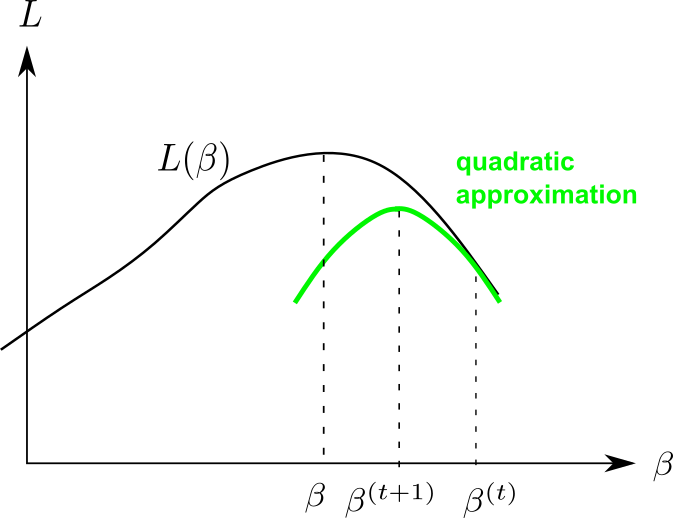
\includegraphics[width=3in]
{gen-lin-mod/gen-lin-mod.png}
\caption{One cycle of Newton-Raphson method
for calculating an estimate $\HAT{\beta}$ for the GLM.}
\label{fig-gml-new-rap}
\end{figure}




\begin{claim}

\beq
\pder{ LL_{\s}}{\beta_{j}}=
 \frac{[y_\s - b'(\xbeta)]}{\av{y_\s, y_\s}}
 \pder{\HAT{\mu}_\s}{\xbeta}
X_{\s, j}
\eeq
\end{claim}
\proof


\beq
\pder{ LL_{\s}}{\beta_{j}}
=
\pder{ LL_{\s}}{\theta_\s}\pder{\theta_\s}{\mu_\s}
\pder{\HAT{\mu}_\s}{\xbeta}\pder{\xbeta}{\beta_{j}}
\eeq

\beq
\pder{ LL_{\s}}{\theta_\s}  =
\frac{y_\s - b'(\theta_\s)}{a(\phi)}
\eeq

\beq
\pder{\mu_\s} {\theta_\s}
=
b''(\theta_\s) = \frac{\av{y_\s, y_\s}}{a(\phi)}
\eeq

\beq
\pder{\HAT{\mu}_\s}{\xbeta} =
(g^{-1})'(\xbeta)
\eeq

\beq
\pder{\xbeta}{\beta_{j}}= X_{\s, j}
\eeq

\beq
\pder{ LL_{\s}}{\beta_{j}}
=
\frac{[y_\s - b'(\theta_\s)]}{\av{y_\s, y_\s}}
 \pder{\HAT{\mu}_\s}{\xbeta}
X_{\s, j}
\eeq

 \qed



\begin{claim}
(Asymptotic expression
for $\av{\HAT{\beta},\HAT{\beta}^T}$
for GLM)


\beq
\av{\HAT{\beta},\HAT{\beta}^T}
\rarrow \cali^{-1}\quad   \text{(asymptotic covariance)}
\eeq
(Hence, more information $\cali$ yields a smaller variance.)
where

\beq
\cali = X^T W X
\eeq
and

\beq
W_{\s, \s'} = \left[\left(\pder{\HAT{\mu}}{\xbeta} \right )^2
\frac{\delta(\s, \s')}
{\av{y_\s, y_\s} } \right]_{\beta=\HAT{\beta}}
\eeq
$\cali$ is called the {\bf information matrix}.

\end{claim}
\proof

\begin{align}
\av{\pder{ LL_\s}{\beta_ { j}}
\pder{ LL_\s}{\beta_ { j'}} }
&=
\av{
\frac{[y_\s - b'(\xbeta)]}{\av{y_\s, y_\s}}
 \pder{\HAT{\mu}_\s}{\xbeta}
X_{\s, j}
\frac{[y_\s - b'(\xbeta)]}{\av{y_\s, y_\s}}
 \pder{\HAT{\mu}_\s}{\xbeta}
X_{\s, j'}
}
\\
&=
 \left[\pder{\HAT{\mu}_\s}{\xbeta}\right]^2
\frac{X_{\s, j} X_{\s, j'}}{\av{y_\s, y_\s}}
\end{align}

\beq
\sum_{\s}
\av{\pder{ LL_{\s}}{\beta_ { j}}
\pder{ LL_{\s}}{\beta_ { j'}} }
=
(X^T W X)_{j, j'}
\eeq
By Section \ref{sec-ent-like-connect}, we have
\beq
\av{\frac{\partial^2 LL_\s}{\partial\beta_ { j}\partial\beta_ { j'}} }
=
-\av{\pder{ LL_\s}{\beta_ { j}}
\pder{ LL_\s}{\beta_ { j'}} }
\eeq
Summing both sides of the last equation over $\s$, we find

\beq
\av{\frac{\partial^2 LL}{\partial\beta_ { j}\partial\beta_ { j'}} }
=
-(X^T W X)_{j, j'}
\eeq
According to  Section \ref{sec-ent-like-connect}, we have
\beq
\av{\HAT{\beta}, \HAT{\beta}^T}\rarrow (X^T W X)^{-1}
\eeq

\qed
